%==============================================================================
% introduction.tex
%==============================================================================

\chapter{Introduction}
\label{chap:introduction}

Intervals \cite{Matsakis2009b} are a new, higher-level primitive for
parallel programming with which programmers directly construct the
program schedule. They are under active development at ETH Zürich as
part of the PhD research of Nicholas Matsakis \cite{Matsakis2010}.

The intervals implementation in Java uses a work-stealing scheduler in
which a worker that runs out of work tries to ``steal'' work from
others. The goal of this thesis is to improve the efficiency of the
intervals scheduler.

\section{Intervals}
\label{sec:intro-intervals}

Existing primitives for synchronizing the control-flow of parallel
threads, such as signals and barriers, are low-level and dangerous to
use. They require careful attention to implementation details to
achieve good performance, and they are prone to errors, particularly
deadlocks and race conditions.

Intervals are a higher-level alternative that make parallel
programming safer while retaining the flexibility and efficiency of
threads. In the Intervals model, users create lightweight tasks and
order them using explicit \emph{happens before} relations
\cite{Lamport1978}. Users need not specify when a thread should block
or acquire a lock. Instead they specify when a task should execute
relative to other tasks, and what locks it should hold when it
executes. The details of making this schedule pass are left to the
runtime system.

The intervals API supports arbitrary \emph{happens before} relations
making the model very flexible. Intervals can be used to emulate
existing thread primitives \cite{Matsakis2009b}, but they can also be
used to easily create program schedules for which no standard thread
primitives exist, such as peer-to-peer synchronization.

One of the primary goals in developing intervals is that program
errors should not lead to deadlocks. This includes both misuse of the
APIs but also miscellaneous errors which causes tasks to abort
unexpectedly, such as dereferencing a null pointer
\cite{Matsakis2009}. A further goal is that an error in one task
should prevent other, dependent tasks from executing
\cite{Matsakis2010a}.

\subsection{Model}
\label{sec:intro-intervals-model}

Intervals are first-class objects in the programming language that
represent the slice of program time used to execute a parallel
task. Intervals are structured hierarchically in a tree. The root of
the interval tree represents the entire program execution. Program
execution itself begins in a child of the root interval.

The conceptual model for intervals consists of points in time ordered
by a \emph{happens before} relation. In the model, an interval
\lstinline|i| consists of a pair of points -- \lstinline|i.start| and
\lstinline|i.end| -- called the start and end point. The start point
represents the moment when the interval begins execution. The end
point represents the moment when the interval's task is
completed. Programmers may introduce arbitrary ordering constraints by
adding \emph{happens before} edges between the start or end points of
different intervals. An edge \lstinline|p1 $\rightarrow$ p2| indicates
that the point \lstinline|p1| must occur before the point
\lstinline|p2|. It also indicates that any memory writes which
\emph{happen before} \lstinline|p1| must be visible to \lstinline|p2|.

An interval can be associated with one or more locks. The intervals
runtime will automatically acquire those locks before the interval's
start point occurs and release them after its end point has occurred.

When an interval executes, it begins by invoking the sequential method
\lstinline|run()|. \lstinline|run()| may either perform the task
directly or create a number of subintervals to achieve the task in
parallel. These subintervals begin to execute once the
\lstinline|run()| method has completed and they are ready to run. A
subinterval is ready to run when it could execute without violating
the \emph{happens before} relation. It will be executed when it is
ready and acquired all its locks.

\begin{figure}[htb]
  \centering
  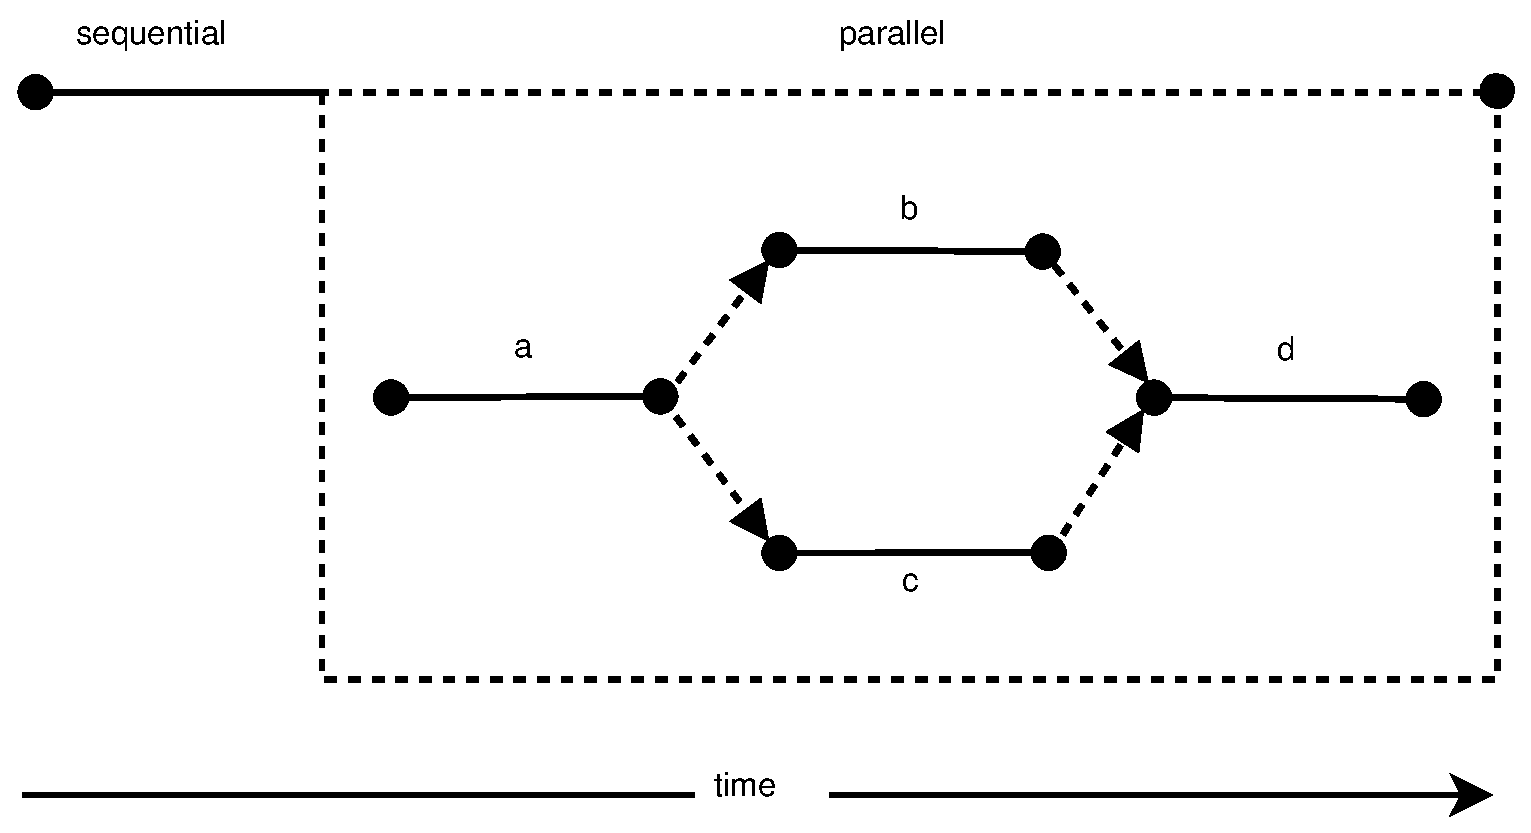
\includegraphics[width=0.96\textwidth]{introduction/interval-graph}
  \caption[Example interval graph]{Example interval graph: Showing an
    interval and its subintervals \lstinline|a|, \lstinline|b|,
    \lstinline|c| and \lstinline|d|.}
  \label{fig:interval-graph}
\end{figure}

The interval model can be depicted as a graph, as shown in Figure
\ref{fig:interval-graph}. The graph contains a single interval with
four subintervals, \lstinline|a|, \lstinline|b|, \lstinline|c| and
\lstinline|d|. The start and end points of each interval are
represented as opaque circles. The subintervals of an interval are
enclosed in a dashed box. This dashed box is omitted for leaf
intervals.

The dashed edges connecting different points indicate user-specified
additions to the \emph{happens before} relation. For example, the end
of \lstinline|a| \emph{happens before} the start of \lstinline|b| and
\lstinline|c| and the ends of \lstinline|b| and \lstinline|c| both
\emph{happen before} the start of \lstinline|d|.

\subsection{Java API}
\label{sec:intro-intervals-java-api}

In the Java API, intervals are represented as instances of the
abstract class \lstinline|Interval| (Listing
\ref{lst:interval-class}). \lstinline|Interval| provides immutable
fields to access the interval's start point, end point, and parent,
along with an abstract \lstinline|run()| method which must be
redefined in a concrete subtype.

\begin{lstlisting}[
  style=FloatNumbers, 
  caption={[\lstinline{Interval} class] \lstinline{Interval}: Serves as the base class for all intervals},
  label=lst:interval-class
]
public abstract class Interval {
  public final Interval parent;
  public final Point start;
  public final Point end;

  protected abstract void run();
}
\end{lstlisting}

Listing \ref{lst:interval-graph} contains Java code which uses the
Intervals API to construct the graph shown in Figure
\ref{fig:interval-graph}.

\begin{lstlisting}[
  style=FloatNumbers, 
  caption={[Intervals Java API example] Code to produce the sample interval graph shown in Figure \ref{fig:interval-graph}},
  label=lst:interval-graph
]
public class ExampleInterval extends Interval {
  public ExampleInterval(Dependency dep, String name) {
    super(dep, name);
  }
  
  protected void run() {
    // Task
  }
  
  public static void main(String[] args) {
    Intervals.inline(new VoidInlineTask() { //*\label{lst:interval-graph-inline-start}
      public void run(Interval start) {
        Interval a = new ExampleInterval(start, "a"); //*\label{lst:interval-graph-new-start}
        Interval b = new ExampleInterval(start, "b");
        Interval c = new ExampleInterval(start, "c");
        Interval d = new ExampleInterval(start, "d"); //*\label{lst:interval-graph-new-end}
        
        Intervals.addHb(a, b); //*\label{lst:interval-graph-add-hb}
        Intervals.addHb(a, c);
        Intervals.addHb(b, d);
        Intervals.addHb(c, d);
        Intervals.schedule(); //*\label{lst:interval-graph-schedule}
      }
    }); //*\label{lst:interval-graph-inline-end}
  }
}
\end{lstlisting}

\subsubsection{Creating Intervals}
\label{sec:intro-intervals-creating-intervals}

To start program execution, the programmer has to create a new child
of the root interval. One could for example use an inline interval to
do so. Inline intervals execute a task during the current interval and
do not return until the task has completed.

Lines \ref{lst:interval-graph-inline-start} --
\ref{lst:interval-graph-inline-end} create the inline subinterval
\lstinline|start| by providing an anonymous task class redefining its
\lstinline|run()| method. \lstinline|start| has four subintervals,
\lstinline|a|, \lstinline|b|, \lstinline|c| and \lstinline|d|. They
are created on lines \ref{lst:interval-graph-new-start} --
\ref{lst:interval-graph-new-end} and are normal, non-blocking
intervals.

\subsubsection{Scheduling Intervals}
\label{sec:intro-intervals-scheduling-intervals}

Newly constructed intervals become eligible for execution once the
\lstinline|schedule()| method is invoked, as shown on line
\ref{lst:interval-graph-schedule} in Listing
\ref{lst:interval-graph}. This gives the user the opportunity to
construct any required dependencies or perform other
initialization. For example, adding the edge
\lstinline|a $\rightarrow$ b| on line \ref{lst:interval-graph-add-hb}
would be unsafe if \lstinline|b| could begin immediately, as it would
be possible that \lstinline|b.start| had already occurred before the
call to \lstinline|addHb()| could add the new dependency.

Explicit calls to \lstinline|schedule()| are unusual, however. This is
because the runtime automatically invokes \lstinline|schedule()| when
the \lstinline|run()| method of an interval returns.


\section{Work-stealing Scheduler}
\label{sec:intro-work-stealing-scheduler}

\todo[inline]{Finish description of work-stealing scheduler}

The implementation of Intervals for Java makes use of a work-stealing
scheduler similar to those found in Cilk \cite{Blumofe1995} or Java 7
\cite{Lea2006} but extended to support locks and happens before
edges. Each worker is implemented as a separate Java thread. The JVM
used to benchmark the implementation is Sun Hotspot JDK 1.6 (see
Appendix \ref{chap:experimental-setup} for information about the
experimental setup).

\subsubsection{SLAW: a Scalable Locality-aware Adaptive Work-stealing
  Scheduler \cite{Guo2010}}

Work-stealing runtime schedulers are increasing in popularity as
scheduling algorithms for dynamic task parallelism, as evidenced by
past work e.g., Cilk \cite{Frigo1998}, Intel Threading Building Blocks
(TBB) \cite{Reinders2007, Contreras2008}, Java's Fork-join Framework
\cite{Lea2000, Lea2000a}, Microsoft Task Parallel Library
\cite{Leijen2009}, and StackThreads/MP \cite{Taura1999}.

A work-stealing scheduler employs a fixed number of threads called
workers. Each worker has a local deque to store tasks. When a worker
is suspended at a synchronization point and there is no local task,
the worker will try to steal from the top of other busy workers'
deque. For a busy worker, tasks are pushed and popped from the bottom
of the deque and these operations are synchronization-free.

\subsubsection{Limits of work-stealing scheduling \cite{Vrba2009}}

A work-stealing scheduler maintains for each CPU (kernel-level thread)
a queue of ready processes waiting for access to the processor. Then,
each thread takes ready processes from the front of its own queue, and
also puts unblocked processes at the front of its queue. When the
thread's own run queue is empty, the thread steals a process from the
back of the run-queue of a randomly chosen thread. The thread loops,
yielding the CPU before starting a new iteration, until it succeeds in
either taking a process from its own queue, or in stealing a process
from another thread. All queue manipulations run in constant-time
($O(1)$), independently of the number of processes in the queues.

The reasons for accessing the run queues at different ends are several
\cite{Frigo1998}:
\begin{enumerate}
\item it reduces contention by having stealing threads operate on the
  opposite end of the queue than the thread they are stealing from;
\item it works better for parallelized divide-and-conquer algorithms
  which typically generate large chunks of work early, so the older
  stolen task is likely to further provide more work to the stealing
  thread;
\item stealing a process also migrates its future workload, which
  helps to increase locality.
\end{enumerate}

The original work-stealing algorithm uses non-blocking algorithms to
implement queue operations \cite{Arora2001}. However, we have decided
to simplify our scheduler implementation by protecting each run queue
with its own lock. We believed that this would not impact scalability
on our machine, because others \cite{Saha2007} have reported that even
a single, centralized queue protected by a single, central lock does
not hurt performance on up to 8 CPUs, which is a decidedly worse
situation for scalability as the number of CPUs grows. Since we use
locks to protect the run queues, and our networks are static, our
implementation does not benefit from the first two advantages of
accessing the run queues at different ends.  Nevertheless, this helps
with increasing locality: since the arrival of a message unblocks a
proces, placing it at the front of the ready queue increases
probability that the required data will remain in the CPU's caches.

Intel's Intel Threading Building Blocks (TBB) \cite{Reinders2007,
  Contreras2008} is a C++ library which implements many parallel
data-structures and programming patterns. TBB's internal execution
engine is also based on work-stealing, and it uses a non-blocking
queue which employs exponential backoff in case of
contention. However, the scheduler is limited to executing only
fully-strict computations, which means that a process must run to
completion, with the only allowed form of blocking being waiting that
children processes exit.3 Thus, the TBB scheduler is not applicable to
running unmodified process networks, where processes can block on
message send or receive.

\subsubsection{The Performance of Work Stealing in Multiprogrammed
  Environment \cite{Blumofe1998a} and Hood: A user-level threads
  library for multiprogrammed multiprocessors \cite{Blumofe1998}}

The work-stealing algorithm dynamically assigns threads to processes
for execution in a provably efficient manner \cite{Blumofe1995,
  Blumofe1999}. In this section, we review the work-stealing
algorithm, and we state the proven performance bounds. In addition, we
describe the non-blocking implementation of this algorithm
\cite{Arora2001}. In the next few sections, we experiment with
applications that are coded to use this non-blocking work stealer.

\minisec{The work-stealing algorithm}

In the work-stealing algorithm, each process maintains its own pool of
ready threads from which it obtains work, and when a process finds
that its pool is empty, it becomes a thief and steals a thread from
the pool of a victim process chosen at random. Each process's pool is
maintained as a double-ended queue, or deque, which has a bottom and a
top. To obtain work, a process pops the ready thread from the bottom
of its deque and commences executing that thread. The process
continues to execute that thread until the thread either blocks or
terminates, at which point the process goes back to the bottom of its
deque to pop off another thread upon which it can work. During the
course of executing a thread, if the thread creates a new thread or
unblocks a blocked thread, then the process pushes the newly ready
thread onto the bottom of its deque.  Thus, so long as a process's
deque is not empty, the process manipulates its deque in a LIFO
(stack-like) manner.

When a process goes to obtain work by popping a thread off the bottom
of its deque, if it finds that its deque is empty, then the process
becomes a thief. It picks a victim process at random (using a uniform
distribution) and attempts to obtain work by removing the thread at
the top of the victim process's deque.  If the victim process's deque
is empty, then the thief picks another victim process and tries
again. The thief repeatedly attempts to steal until it finds a victim
whose deque is non-empty, at which point the thief reforms and
commences work on the stolen thread as described above. Since steals
take place at the top of the victim's deque, stealing operates in a
FIFO manner.

\subsubsection{A Java fork/join framework \cite{Lea2000}}

The heart of a fork/join framework lies in its lightweight scheduling
mechanics. FJTask adapts the basic tactics pioneered in the Cilk
work-stealing scheduler:

\begin{itemize}
\item Each worker thread maintains runnable tasks in its own
  scheduling queue.
\item Queues are maintained as double-ended queues (i.e., deques,
  usually pronounced ``decks''), supporting both LIFO push and pop
  operations, as well as a FIFO take operation.
\item Subtasks generated in tasks run by a given worker thread are
  pushed onto that workers own deque.
\item Worker threads process their own deques in LIFO (youngest-first)
  order, by popping tasks.
\item When a worker thread has no local tasks to run, it attempts to
  take (``steal'') a task from another randomly chosen worker, using a
  FIFO (oldest first) rule.
\item When a worker thread encounters a join operation, it processes
  other tasks, if available, until the target task is noticed to have
  completed (via isDone). All tasks otherwise run to completion
  without blocking.
\item When a worker thread has no work and fails to steal any from
  others, it backs off (via yields, sleeps, and/or priority
  adjustment) and tries again later unless all workers are known to be
  similarly idle, in which case they all block until another task is
  invoked from top-level.
\end{itemize}

\missingfigure{Illustrate push, pop and steal}

As discussed in more detail in \cite{Frigo1998}, the use of LIFO rules
for each thread processing its own tasks, but FIFO rules for stealing
other tasks is optimal for a wide class of recursive fork/join
designs. Less formally, the scheme offers two basic advantages:

It reduces contention by having stealers operate on the opposite
side of the deque as owners. It also exploits the property of
recursive divide-and-conquer algorithms of generating ``large''
tasks early. Thus, an older stolen task is likely to provide a
larger unit of work, leading to further recursive decompositions
by the stealing thread.

As one consequence of these rules, programs that employ
relatively small task granularities for base actions tend to run
faster than those that only use coarse-grained partitioning or
those that do not use recursive decomposition. Even though
relatively few tasks are stolen in most fork/join programs,
creating many fine-grained tasks means that a task is likely to
be available whenever a worker thread is ready to run it.

\subsubsection{Programming with Intervals \cite{Matsakis2009b}}

Coroutines \cite{Conway1963} and continuations \cite{Reynolds1993} are
two building blocks for manipulating control-flow in a sequential
context. Either would make a useful primitive on which to build the
intervals library and would provide an alternative to rewriting
programs in an event-oriented style.

Futures are annotations for parallel execution which act similarly to
a lazy or deferred execution. Expressions annotated as being safe for
parallel execution are executed in parallel; when the program reaches
a point where the result of the expression is needed, the main thread
blocks until the evaluation of the expression has completed. Futures
were first implemented for MULTILISP \cite{Halstead1985} but have
since been ported to a number of other languages, including Java
\cite{Navabi2008}.  Futures can be seen as a subset of intervals that
lack the extended happens before relationships. Furthermore, most
implementations of futures make no guarantees with respect to
deadlock-freedom or other safety properties.

Cilk \cite{Blumofe1995, Frigo1998} and JCilk \cite{Danaher2005} are
supersets of C and Java respectively which add support for
parallelism, primarily in the form of fork-join or barrier style
computations. Cilk pioneered many of the dynamic scheduling and work
stealing techniques used in the intervals implementation itself.

Jade \cite{Rinard1998} uses programmer-provided specifications to
dynamically parallelize a program. Shared objects were specially
integrated into the type system. Tasks declare those objects that they
affect and how; adherence to these declarations is checked
dynamically. The ability for intervals to be associated with locks
works in a similar fashion, but Jade did not attempt to model happens
before relationships in its task specifications.

X10 \cite{Charles2005, Saraswat2010} introduced a number of innovative
synchronization constructs. The most recent, phasers
\cite{Shirako2008, Shirako2010}, are a combination of barriers and
signals. Threads wishing to synchronize with one another make use of a
shared phaser object.  Threads indicate how they will use a phaser by
placing it into different modes, such as signal-wait-next or
wait-only, that grant different capabilities. A combination of static
and dynamic safety checks ensures that programs cannot be deadlocked
through using a phaser. When synchronizing on a barrier, a special
“single” mode allows a small section of code to be executed by a
single thread before the waiting threads resume. Intervals can be used
to perform the same kinds of synchronizations as phasers and with
similar safety guarantees. However, intervals are a standalone
mechanism that also replaces threads, thread joins, and integrates
locks, all of which are beyond the scope of phasers. On the other
hand, phasers are closer to existing threading primitives and
therefore can be adopted more easily.

OpenMP \cite{OpenMP2008} and the Message Passing Interface (MPI)
\cite{MPI2009} are two higher-level alternatives to threads for
writing parallel programs. Unlike intervals, they are focussed on SIMD
programming, although both can be used more generally.

JSR166 \cite{Lea2004} introduced a number of concurrency-related
utility classes to Java, including futures, thread pools, read-write
locks, and concurrent containers such as maps and queues. Java 7 will
likely contain additional classes \cite{Lea2006}, among them the
fork-join framework that intervals itself is built upon. For C\#, the
Parallel Extensions \cite{Leijen2009} library promises a similar
lightweight task framework.  Neither of these frameworks includes any
mechanism for declarative or explicit happens before relationships;
instead, users use traditional joins to wait for tasks to complete.

Apple's Cocoa framework includes a class NSOperation \cite{Apple2008}
that is similar to intervals. Like an Interval, each NSOperation
embodies a particular task, and a user may declaratively specify that
one operation cannot execute until another has finished (the
equivalent of a startAfterEndOf() dependency). Unlike intervals,
however, NSOperations do not permit other kinds of dependencies nor
are they integrated with locks. This means that they cannot easily be
used to describe the patterns in this paper, with the exception of
point to point synchronization.

The Java Memory Model \cite{Manson2005} defines how parallel threads in
Java interact with shared memory. In addition to defining formally
what it means for a Java program to be correctly synchronized, it
describes the legal behaviors of incorrectly synchronized programs
which include data races. In the Java Memory Model, happens before
relationships potentially result from imperative actions such as
acquiring locks, accessing volatile fields, or joining a thread. This
model can be easily adapted to the explicit happens before
relationships used by intervals. When using our data race analysis,
however, there is no need to define the semantics of incorrectly
synchronized programs, because they cannot occur.

\subsubsection{Handling Errors in Parallel Programs Based on Happens
  Before Relations \cite{Matsakis2010a}}

Erlang \cite{Erlang2010} embodies a strict share-nothing philosophy,
in which actors with disjoint heaps communicate with messages. The
simplicity of this approach is appealing, but we believe there are
many scenarios where shared memory is an easier and better choice,
given the right tools.

Cilk \cite{Blumofe1995, Frigo1998} and OpenMP 3.0 \cite{OpenMP2008}
both offer lightweight task frameworks where tasks are executed in a
tree structure.  Tasks in these languages are not first-class objects,
however, and they do not support arbitrary dependency graphs. Java's
Fork-Join Framework \cite{Lea2006, Lea2000, Lea2000a} and Intel's
Threading Building Blocks (TBB) \cite{Reinders2007, Contreras2008}
both offer a more flexible alternative, but lack a higher-level
interface to task dependencies. The fork-join framework permits
lightweight tasks to be joined, and TBB allows tasks to delay starting
until an associated counter is decremented to zero.

The parallel extensions for .NET \cite{Leijen2009} offer a task
library with a similar feeling to intervals. In addition to the usual
join-based task routines, they also permit tasks to have
continuations, which are dependent tasks that execute and are given
the result of the previous task to begin (the equivalent of edges from
the end of one interval to the start of another). This approach is
powerful but does not permit the full range of happens before edges
supported by intervals.

X10 \cite{Charles2005, Saraswat2010} offers a revised threading model
which includes a number of innovative synchronization
constructs. Among them are phasers \cite{Shirako2008, Shirako2010}, a
combination of barriers and signals which can guarantee data-race
freedom. Intervals can be used to construct the same patterns as
phasers with similar guarantees, but also go further by replacing
thread joins and other constructs in the X10 toolset.

Intervals in Java align nicely with the Java Memory Model
\cite{Manson2005}: The happens before relation defined by intervals
can be seen as a deterministic subset of the full happens before
relation defined by the memory model, which includes edges due to
constructs like volatile fields or synchronized sections.

\todo{Add missing references}

\subsubsection{Missing references}

\begin{itemize}
\item The Performance of Work Stealing in Multiprogrammed Environment
  \cite{Blumofe1998a}
\item Space efficient execution of deterministic parallel programs
  \cite{Simpson1999}
\item Lazy binary-splitting: a run-time adaptive work-stealing
  scheduler \cite{Tzannes2010}
\item Mely: Efficient Workstealing for Multicore Event-Driven Systems
  \cite{Gaud2010}
\item Limits of work-stealing scheduling \cite{Vrba2009}
\item Helper locks for fork-join parallel programming
  \cite{Agrawal2010}
\item Hood: A user-level threads library for multiprogrammed
  multiprocessors \cite{Blumofe1998}
\item Efficient support for fine-grain parallelism on shared-memory
  machines \cite{Lowenthal1998}
\item Hood: A User-Level Thread Library for Multiprogramming
  Multiprocessors \cite{Papadopoulos1998}
\item Compiler Support for Work-Stealing Parallel Runtime Systems
  \cite{Raman2009}
\end{itemize}


\section{Overview}
\label{sec:intro-overview}

The goal of this thesis is to improve the efficiency of the intervals
scheduler and is divided into the two following parts.

\subsubsection{\autoref{part:queues}. Explore and profile different
  work-stealing queue implementations}

In a work-stealing scheduler, each worker keeps a pool of work items
waiting to be executed. The current intervals implementation uses
doubled-ended queues (deques). In \autoref{part:queues} of this thesis
we explored alternative queue implementations and compared them to the
current implementation.

\todo{Summarize part I}

\subsubsection{\autoref{part:locality}. Locality-aware work-stealing}

Currently the intervals scheduler randomly schedules work items and
when stealing a work item, the worker chooses his victim by random. In
\autoref{part:locality} of the thesis we implemented and analyzed
locality-aware scheduling of intervals. In locality-aware scheduling,
each interval can be given an affinity for a place, and when a worker
belonging to a certain place obtains an interval, it gives priority to
the intervals with affinity for the place.

\todo{Summarize part II}

%%% Local Variables: 
%%% mode: latex
%%% TeX-master: "thesis"
%%% End: 
